%%%%%%%%%%%%%%%%%%%%%%%%%%%%%%%%%%%%%%%%%%%%%%%%%%%%%%%%%%%%%%%%%%%%%%%%%%%%%%%
%%%%%%% ColdADC Testing Results
%%%%%%%%%%%%%%%%%%%%%%%%%%%%%%%%%%%%%%%%%%%%%%%%%%%%%%%%%%%%%%%%%%%%%%%%%%%%%%%

\documentclass[12pt]{article}

\topmargin=-0.5in
\oddsidemargin=0in
\evensidemargin=0in
\textwidth=6.2in
\textheight=9.25in

\usepackage[dvips]{graphics}
\usepackage{rotating}
\usepackage{amssymb,amsmath}
\usepackage{graphicx}
\usepackage{cite}
\usepackage{color}
\usepackage[table]{xcolor}
\usepackage{colortbl}
\usepackage{enumerate}

%% draftwatermark causes infinite loop on SL6's ancient TeXLive
%\usepackage[firstpage]{draftwatermark}
\usepackage{lipsum}
\usepackage{tikz}

\usepackage[T1]{fontenc}
\usepackage[utf8]{inputenc}
\usepackage[blocks,affil-it]{authblk}

\RequirePackage{lineno}

\bibliographystyle{plain}
\bibliographystyle{unsrt}

\usepackage{graphicx, subfigure}
\usepackage[colorlinks=true,urlcolor=black,linkcolor=black,citecolor=black,bookmarks=true]{hyperref}

\setcounter{tocdepth}{2}



\begin{document}
%\linenumbers

\title{DUNE ColdADC ASIC Preliminary Testing Results}

%\date{\today}
\date{January 10, 2020}
\author{Authors go here}
%	\input{150606_authors}
%	\input{authors_template}

\maketitle

\centerline{DUNE Electronics Consortium}

%\SetWatermarkText{DRAFT}
%\SetWatermarkLightness{0.8}
%\SetWatermarkScale{5}


\begin{abstract}
Abstract
\end{abstract}


\newpage
\tableofcontents

\newpage

%%%%%%%%%%%%%%%%%%%%%%%%%%%%%%%%%%%%%%%%%%%%%%%%%%%
\section{Introduction [{\color{red} Grace/Lin}] }
%\section{Introduction}
\label{sec:1}

The DUNE ColdADC is a digitizer ASIC intended for operation in the Deep Underground Neutrino Experiment (DUNE) Far Detectors. It will operated immersed in Liquid Argon (LAr) and will need to operate reliably, without any servicing or component replacement, for over 30 years at a temperature of 87 K.

The ColdADC was implemented in 65 nm CMOS by a team comprised of engineers from Fermilab (FNAL), Brookhaven National Laboratory (BNL), and Lawrence Berkeley National Laboratory (LBNL). The prototype was submitted for fabrication in late 2018 and received in early 2019. Evaluation is ongoing. 

The first prototype meets essential requirements. The key performance specification, noise, is as expected. The prototype is currently being integrated into a new revision of the DUNE Far Detector Front-End Mother Board (FEMB). Preliminary results are good, and the DUNE Far Detector FEMB is displaying better noise performance than the SBND FEMB, which uses a Commercial Off-the-Shelf (COTS) ADC. This enables the use of a lower gain setting in LArASIC and thus larger dynamic range. The key specifications of the ColdADC compared to the measured results are presented in Table~\ref{tab:coldadc_specs}.
\begin{table}[h]
\centering
\begin{tabular}{|c|c|c|c|}
\hline
\textbf{ Specification } & \textbf{Value} & \textbf{Result} & \textbf{Note}  \\ \hline \hline
Operation Temperature &  RT and 87 K & Success & \\ \hline
Sampling Rate & 2 MHz & 2 MHz & \\ \hline
Noise & 200 $\mu$V-rms & 189 $\mu$V-rms & @ LN$_2$ temp \\ \hline
Differential Non- & $\pm$0.5 LSB (at 12-bit level) & $+0.2$ to $-0.5$ LSB & @LN$_2$ ; typical values \\
linearity (DNL) & & &  \\ \hline
Integral Non- & $\pm$1 LSB (at 12-bit level) & $+1.2$ to $-1.1$ LSB & @LN$_2$, typical values \\
Linearity (INL) & & &  \\ \hline
Effective-Number- & 11.0 bits & <mean>=10.6 bits & @ LN$_2$ \\ 
of-Bits (ENOB) & & rms=0.3 bits & \\ \hline
No Missing Codes & N/A & Success & @LN$_2$ and RT \\ 
Across Dynamic Range & & & \\ \hline
Crosstalk  & No Specification & $<1\%$ & \\ \hline
Power Consumption & $<$50 mW/channel(??) & 24 mW/channel &  \\ \hline
\end{tabular}
\caption{Summary of Results}
\label{tab:coldadc_specs}
\end{table}     1000

In order to mitigate the hot carrier effect (and ensure long operational lifetime at 87 K), the circuits in the ColdADC prototype
%To ensure the ColdADC can operate long-term at 87 K, the ASIC was designed using high-reliability principles developed by BNL. 
%Studies conducted by BNL determined that hot electron effects can cause substrate damage in CMOS circuits and these effects 
%are exacerbated by operation at cold temperature. In order to mitigate hot electrons by reducing the magnitude of the electric 
%field at the gate-drain interface, the circuits on the ColdADC prototype 
are designed with a minimum transistor channel 
length 50\% longer than the minimum length allowed by the process, and the power supplies are kept at 10\% below their nominal 
values. To follow this rule, the synthesized digital circuits use a custom standard cell library with longer 
transistors than the foundry-supplied library. In addition, the architecture of the ADC was chosen as the Pipelined ADC, whose 
performance depends primarily on the matching of ratioed capacitors. Studies conducted by BNL showed capacitor performance 
degraded less than active devices under cold conditions. 


%%%%%%%%%%%%%%%%%%%%%%%%%%%%%%%%%%%%%%%%%%%%%%%%%%%


\section{Test Setup}
\label{sec:2}

%%%%%%%%%%%%%%%%%
% Test Setup
%%%%%%%%%%%%%%%%%

\subsection{Cryogenic Test System (CTS) [{\color{red} Lin}] }
\label{sec:2.1}

%%%%%%%%%%%%%%%%
% (LIN) CTS
%%%%%%%%%%%%%%%%

The Cryogenic Test System (CTS) was built by a group from the Michigan State University. The CTS allows the user to thermal cycle the ASIC from room to cryogenic temperature. Figure~\ref{fig:cts} shows the CTS.
\begin{figure}[htb]
\centering
%\begin{minipage}[b]{1.0\textwidth}
\begin{center}
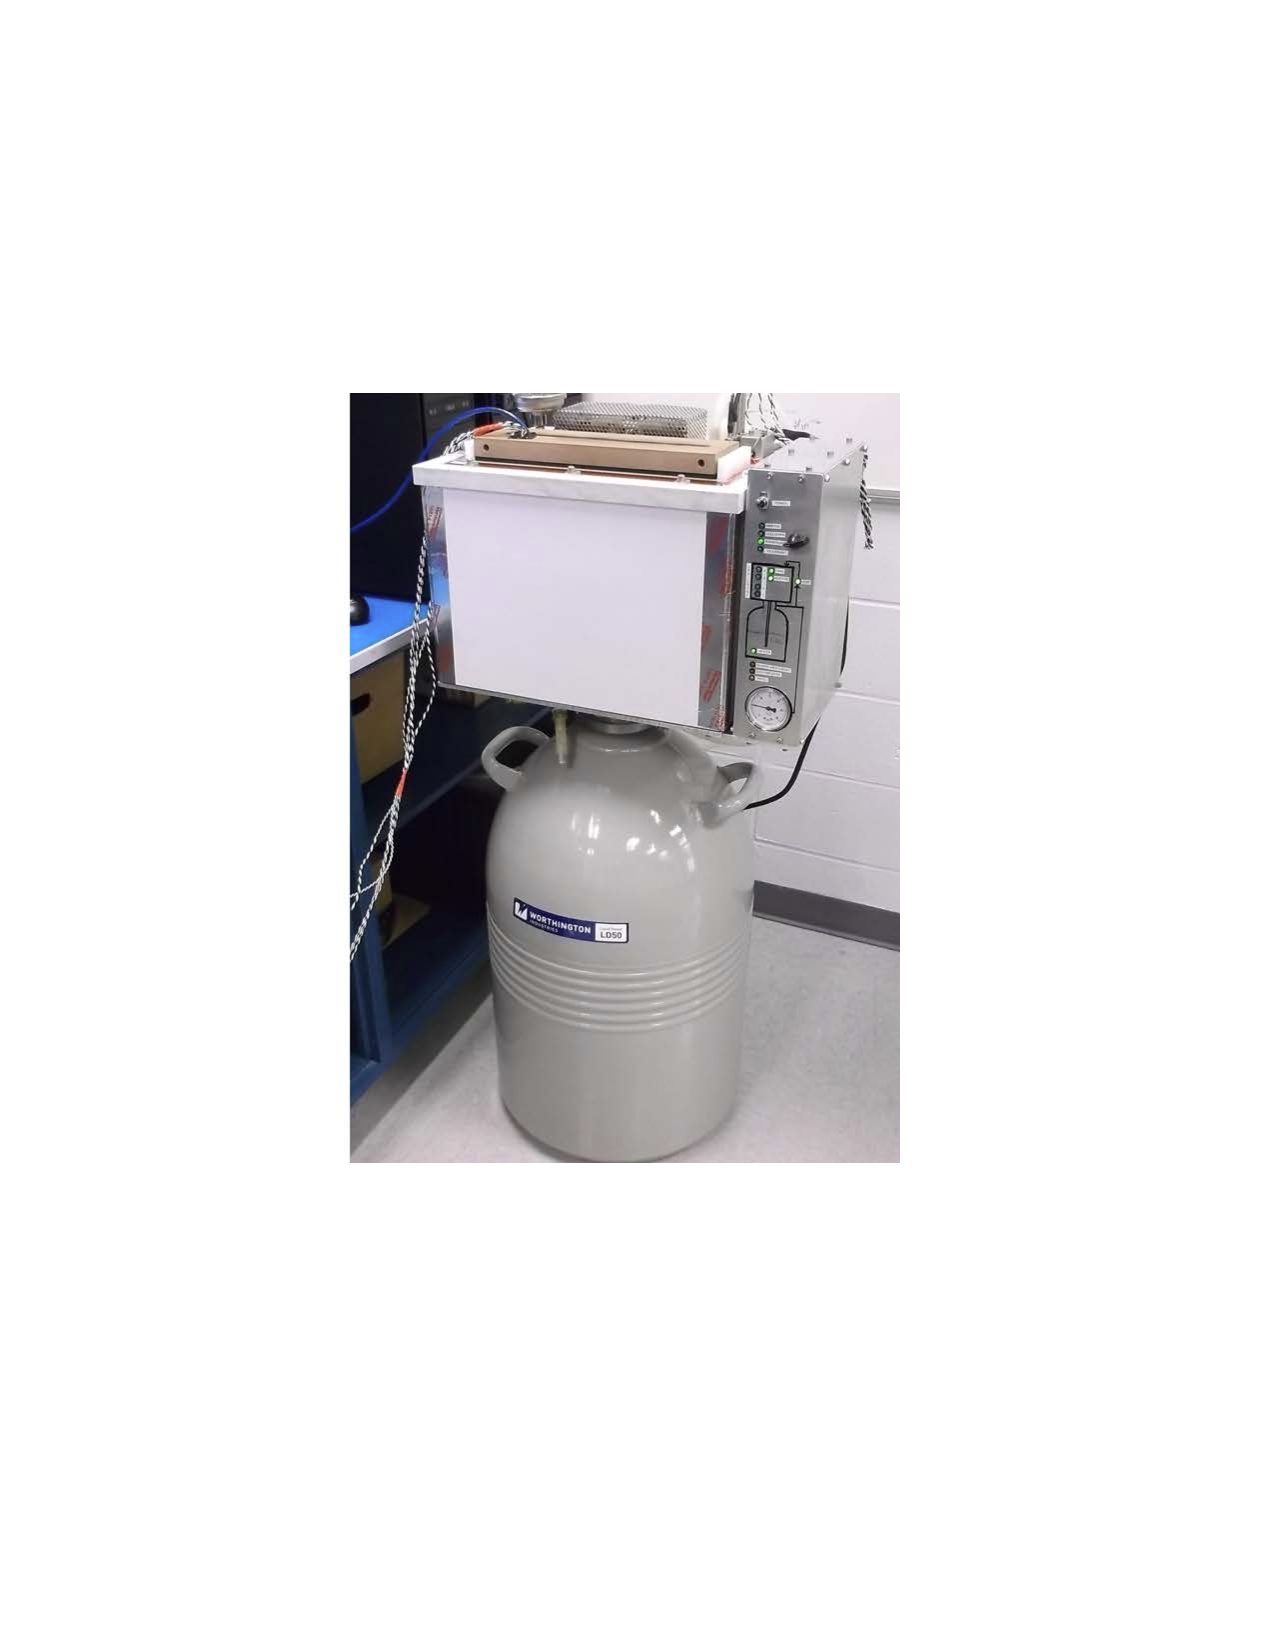
\includegraphics[width=0.5\textwidth]{figures/CTS.pdf}
\end{center}
%\end{minipage}
\caption{Cryogenic Test System.}
\label{fig:cts}
\end{figure}


\subsection{BNL Test System [{\color{red} Gao}] }
\label{sec:2.2}

Describe BNL test setup including the test boards.

\subsection{Fermilab Cryo Cooler Test System [{\color{red} Christian}] }
\label{sec:2.3}
%%%%%%%%%%%%%%%%%%%%%%%%%%%%%%%%%%%%%%%%%%%%%%%%%%%%%%%
%(Christian) Fermilab test setup including the test boards
%%%%%%%%%%%%%%%%%%%%%%%%%%%%%%%%%%%%%%%%%%%%%%%%%%%%%%%
\begin{figure}[htb]
\centering
%\begin{minipage}[b]{1.0\textwidth}
\begin{center}
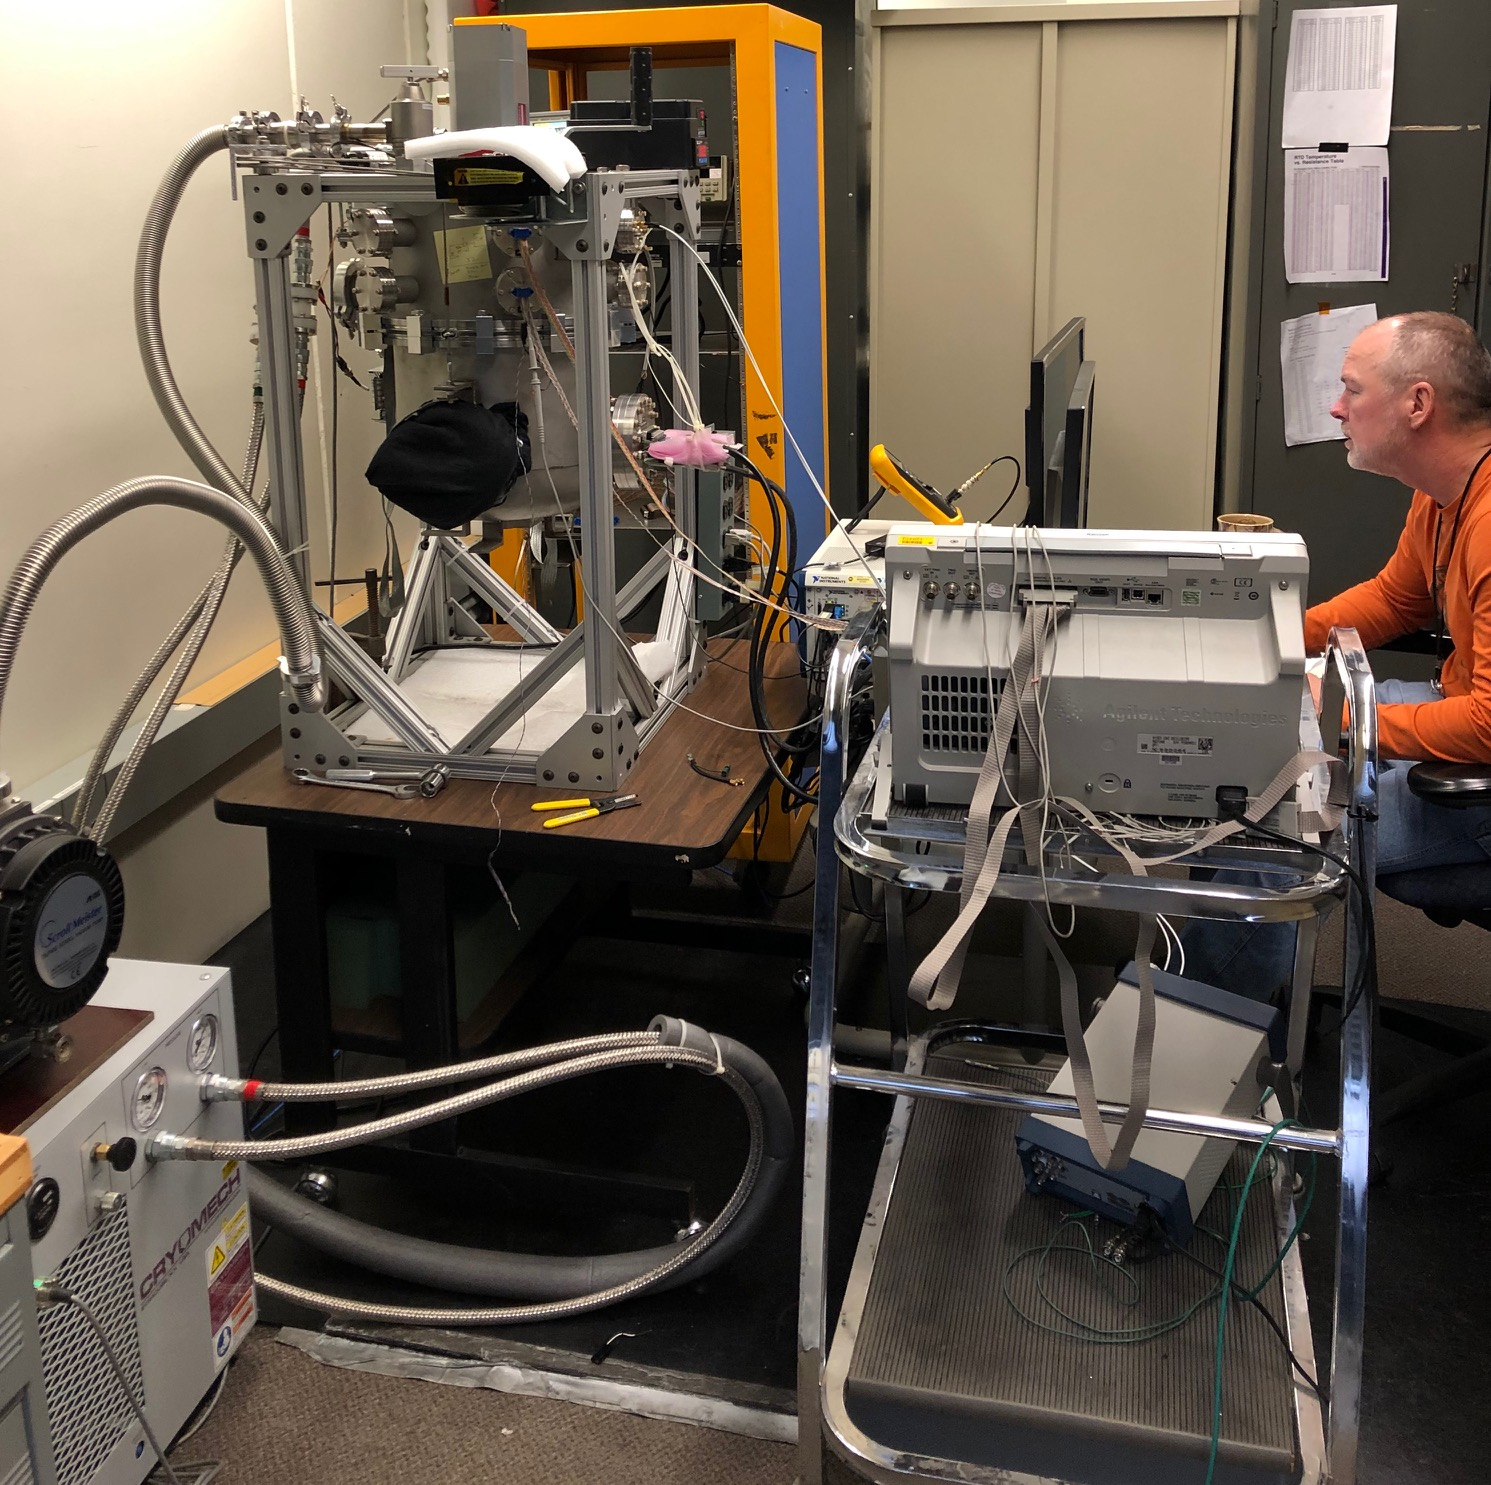
\includegraphics[width=0.95\textwidth]{figures/cryotestsystem.jpg}
\end{center}
%\end{minipage}
\caption{Fermilab Cryocooler Test System.}
\label{fig:cryocoolertestsystem}
\end{figure}

The Fermilab Cryocooler Test System, see Figure~\ref{fig:cryocoolertestsystem}, consists of a vacuum vessel and a cryogenic refrigerator. The cryogenic refrigerator is a Cryomech PT-60.  It is a closed-loop cryocooler consisting of a helium compressor (located next to the vacuum vessel) and a cold head (located on top of the vacuum vessel).  The cryocooler cools a copper cold-plate inside the vacuum vessel to a minimum of 60 K.  A 100 ohm platinum RTD and a 75 Watt heater are mounted on the cold-plate.  A temperature controller cycles the heater on and off to achieve the set-point temperature.  Any temperature between 60 and 250 K can be set.
The vacuum vessel has 2 large penetrations and 12 small penetrations that can be used in device testing.  Typically, one of the large penetrations is used as an inspection port and the other as a feedthrough for ribbon cables.  The small ports allow for a variety of other signal feedthroughs.  

Two printed circuit boards are used in ASIC testing, a ``cold board,'' which is screwed onto the cold-plate and includes a large unmasked copper thermal contact area, and a ``warm board'' which is mounted as a mezzanine board on the cold-board.  RTDs are placed on both the cold board and the warm board.  The temperature on the warm board is typically 100 K higher than than the temperature on the cold board.  If the cryocooler is regulated to hold the cold-board at LN$_2$ temperature, then the temperature on the warm board is $\sim-96^{\circ}$C, which is warm enough for most COTS components to operate properly.

The cold board used in tests of ColdADC includes a single bare chip, wire bonded to the printed circuit board.  An 80-pin header carries digital I/O and three of the four bias voltages (VDDIO and both digital voltages) between the cold board and the warm board.  A 60 pin header carries the analog bias voltage and all analog signals with the exception of the analog inputs to the ColdADC.  Jumpers allow the analog inputs to be grounded or connected to an external sources using cables.  The only other parts on the cold board are bypass capacitors (selected for cryogenic use) and test points.

The warm board includes connectors that mate to the cold board connectors, a 52-pin header used for a cable connection to an National Instruments (NI) FPGA module, single ended to differential converters used for the 64 and 2 MHz clock signals, differential to single ended converters for the LVDS output signals, level shifters for the CMOS I/O signals, passive components, buffer amplifiers, and SMA connectors for the analog outputs, SMA connectors for the ADC test inputs, and 9-pin D connectors for cable connections to NI power supplies that provide source-measure functionality (used for chip power and for providing or measuring analog I/O signals such as reference voltages).

Test software was written using National Instruments LabView and run on a single-crate PXIe system consisting of a controller, an NI 6583 FPGA unit, and 5 power supply modules.  A Keysight 33500B waveform generator was used to provide input signals.  Analog measurements were made using an oscilloscope and a DVM as well as with the NI modules.


\subsection{LBNL Test Board  [{\color{red} Lin}] }
\label{sec:2.4}

%%%%%%%%%%%%%%%%%%%%%%%%%%%%%%%%%%%%%%%%%%%%%%%%%%%%%%%
% Lin and Prakash - LBL test setup
%%%%%%%%%%%%%%%%%%%%%%%%%%%%%%%%%%%%%%%%%%%%%%%%%%%%%%%

\subsubsection {LBNL mother board}

A single board solution was developed by LBNL to test the ColdADC. The mother board accommodates one ColdADC bare die, wire bonded to the board. The mother board is divided into ``cold" and ``warm" sections with an empty strip of PCB in between to clamp the board to CTS. The ColdADC, extremely low noise LDO's which supply four different VDDs to the ColdADC are present in the ``cold section" of the mother board. Power supply distribution circuitry, Spartna 6 FPGA, LDO's for the FPGA, 80MHz oscillator for clocking the FPGA, external unity buffers and 12 bit ADCs to digitize the monitor signals from the ColdADC and 40 pin standard header to connect the Raspberry PI are in the ``warm section" of the mother board. Analog inputs to the ColdADC are supplied by 16 edge-mount SMA connectors. There are two additional edge-mount SMA connectors to supply test inputs directly to the ADC-core. Eight-pin standard header connector is available if there is a need to bypass the ColdADC LDOs and supply external VDDs directly to the ASIC.

Although the mother board is very successful, there are three minor limitations: Due to small block-ram size of the FPGA the ADC data cannot be streamed continuously to the Raspberry PI this makes the calibration and linearity calculation of the ColdADC a time consuming process. Secondly, this version of the mother board is a Chip-On-Board (COB) version, this makes testing more than one ASIC very difficult, replacing an ASIC essentially means destroying the current chip and mount a new chip. Finally, the analog inputs to the ColdADC can only be single ended. Due to the lack of space only 16 SMA connectors were mounted on the board.  

A new three board solution was developed to overcome these three limitations. Version 2 LBNL test setup consists of a motherboard, a daughter card and an FPGA mezzanine board. The daughter card can either designed to have bare die or a packaged chip. A modular approach was taken to design the new test setup. The same test setup can be used for ColdADC V2 chip just by minor re-designing the COB daughter card. The V2 LBNL test setup is shown in Figure \ref{fig:v2_board}. This test board, just like the previous version has ``cold section" and ``warm section". The COB daughter card and the LDOs are at the bottom, in the ``cold" section of the board. The power distribution circuitry, FPGA mezzanine board, and the Raspberry PI are in the ``warm" section of the board. Four 8-pin Samtec 5.00 mm 50 Ohm Ganged Micro-Miniature RF Jack connectors are used to drive external differential or single ended analog inputs to the ColdADC.  

\begin{figure}[h!]
\centering
  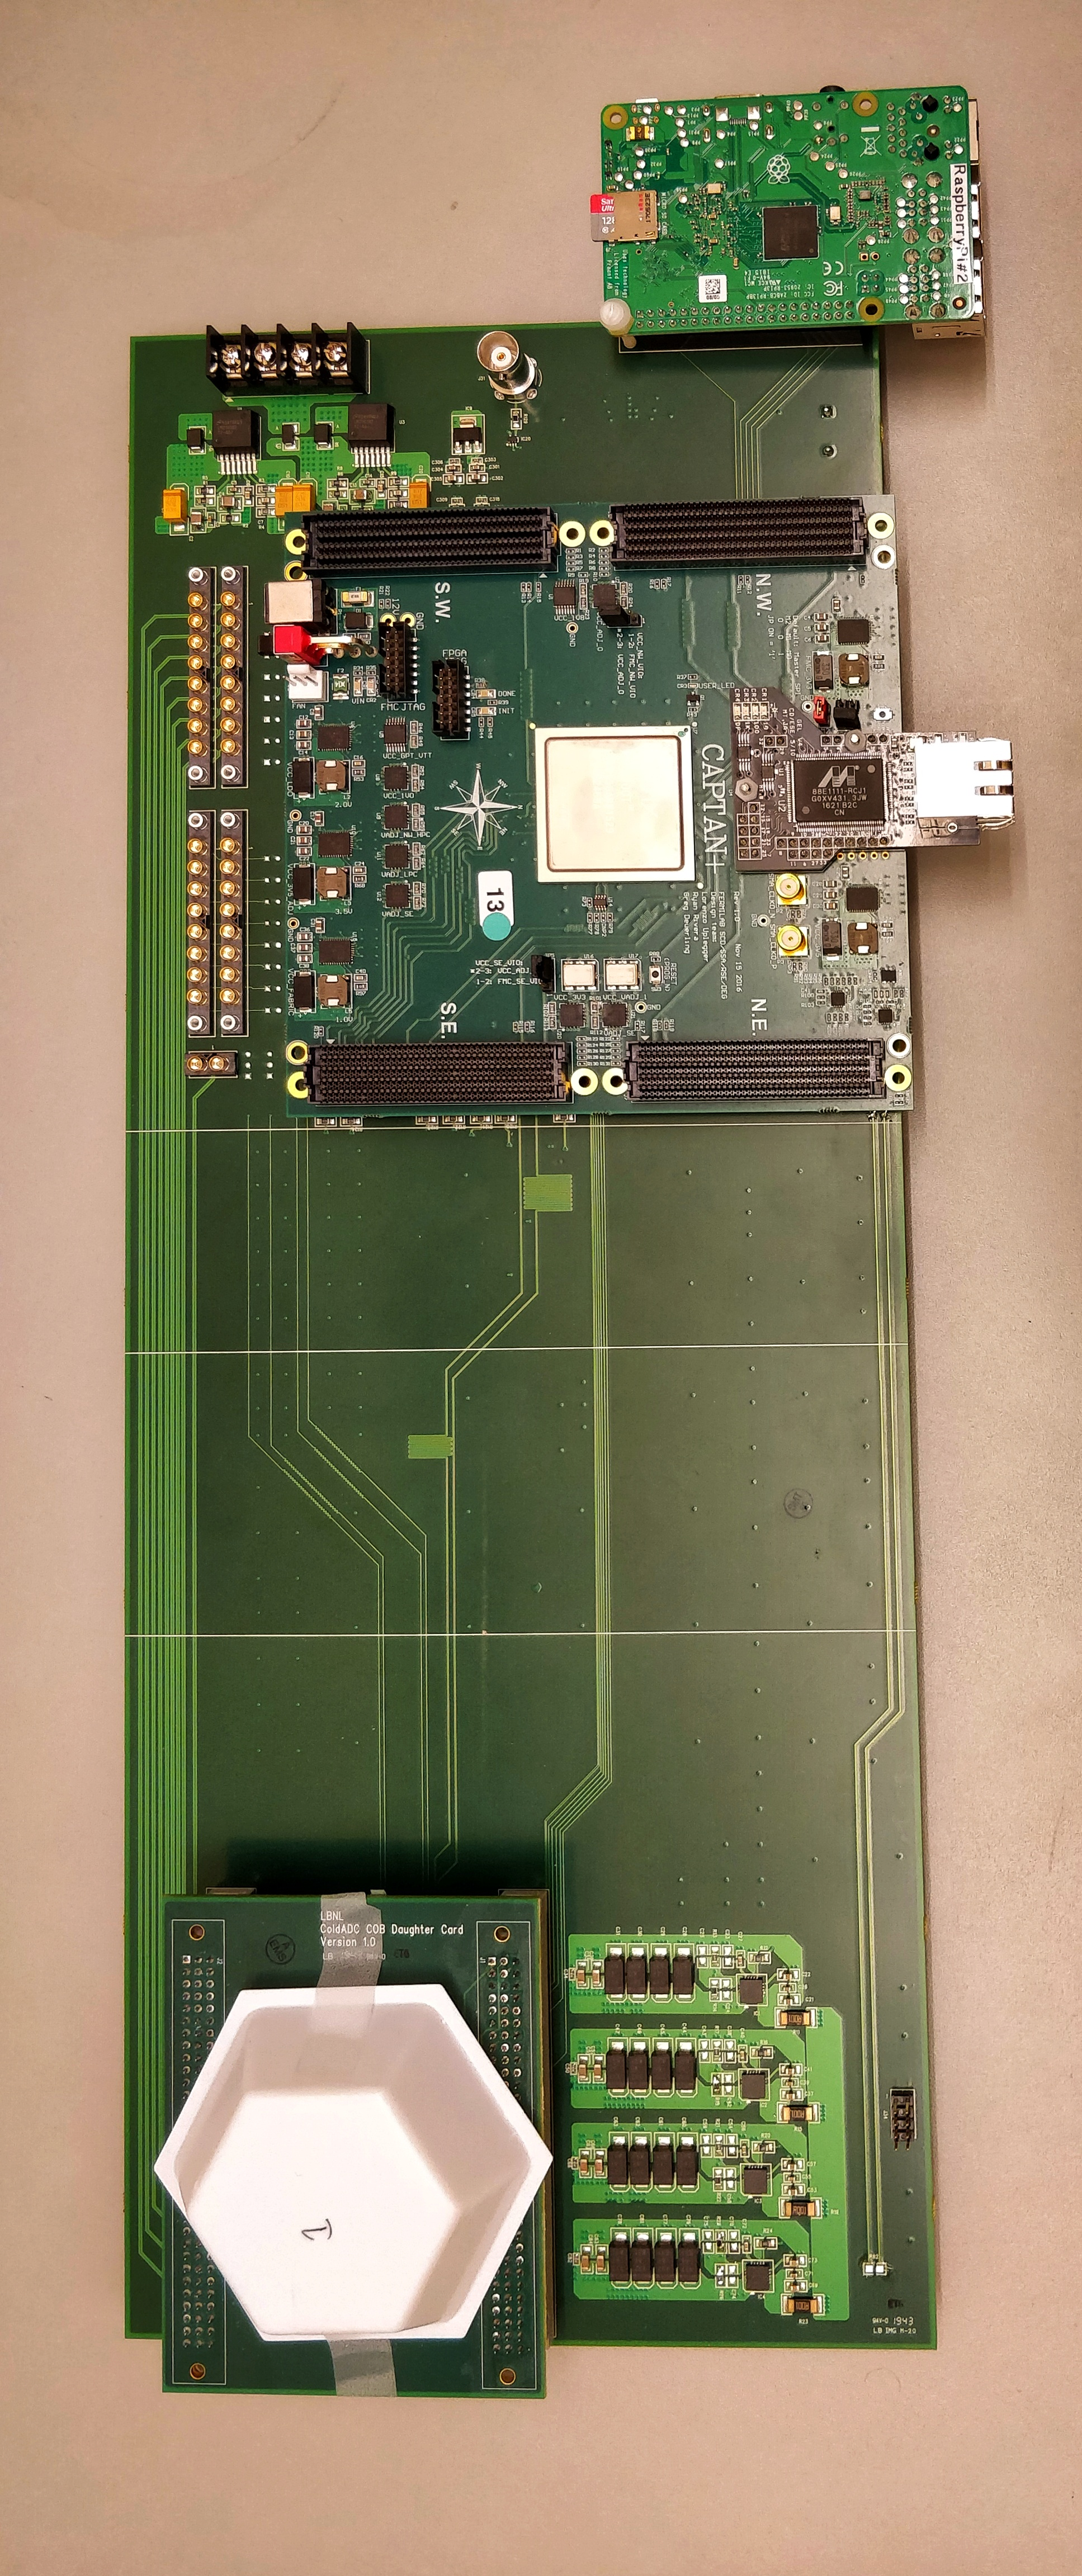
\includegraphics[width=0.3\linewidth]{figures/prakash_fig/v2_board.jpeg}
  \caption[LBNL ColdADC Testboard]{Version 2 LBNL ColdADC Testboard}
  \label{fig:v2_board}
\end{figure}




%%%%%%%%%%%%%%%%%%%%%%%%%%%%%%%%%%%%%%%%%%%%%%%%%%%

\section{Functional Testing [{\color{red} Christian}] }
\label{sec:3}

COLDADC is highly programmable.  Many circuit blocks can be bypassed and two versions of a number of circuit blocks are included to mitigate the risk that one might fail.  Testing at Fermilab concentrated on verifying the functionality of all of the circuit blocks.  Three design errors were revealed and a number of documentation errors were corrected.  The table below summarizes the tests.
 
 \begin{table}[h]
\centering
\begin{tabular}{|c|c|}
\hline
\textbf{ Test/Circuit} & Result  \\ \hline \hline
Power on &  No shorts \\ \hline
I2C & Works as designed (registers can be written and read) \\ \hline
Reset & Works as designed (registers are set to default values) \\ \hline
UART & Works as designed \\ \hline
LVDS I/O & Works as designed (output amplitude controlled as designed) \\ \hline
Clock Generation & 16 MHz clock verified \\ \hline
Data Formatter & Works as designed \\ \hline
Band Gap Reference & Works $\sim$as designed at room temperature, but fails when cold. \\ 
 & Problem traced to a design error (inclusion of the wrong \\ 
 &  OP Amp in the current source DAC); works as designed \\ 
 &  with elevated VDDA2P5 (needs 2.7V at 77K) \\ \hline
 CMOS Reference & Works as designed \\ \hline
 Automatic Calibration & Fails.  Calibration can be done by using control \\ 
  & registers to force the sequence of steps required \\ 
   & and doing arithmetic off-chip.\\ 
    & Eventually we noticed that when automatic calibration is \\ 
     & attempted, the low order bytes of W0 and W2 for every \\ 
      & ``calibrated'' stage are equal. Simulation verified that  \\ 
       & this is due to a timing error storing W0 and W2. \\ \hline
 ADC Correction Logic & Works as designed (loaded fake comparator output \\ 
  & values; resulting ADC output is as expected). \\ \hline
Pipeline ADC & Linear ramp yields close to linear output; \\ 
 & deviation from linear at extremes of ramp; \\ 
  & no significant deviation from linear when cold. \\ \hline
Input buffers & Significant non-linearity observed. \\ 
 & Problem traced to circuit naming confusion that resulted \\ 
 & in level shifters being omitted from input buffers. \\
 & Buffers operate $\sim$as designed with elevated VDDD1P2 \\ \hline
 Sample and Hold and MUX & Require elevated VDDD1P2 because \\ 
 & inputs come through input buffers. \\ \hline
\end{tabular}
\caption{Functional Testing.}
\label{tab:Functionality}
\end{table}
	
%%%%%%%%%%%%%%%%%%%%%%%%%%%%%%%%%%%%%%%%%%%%%%%%%%%

\section{Performance Results}

\subsection{Noise}
\subsubsection{ColdADC Only}
\subsubsection{LArASIC + ColdADC  [{\color{red} Gao}] }

\subsection{Static Linearity (INL,DNL)}

\subsection{Dynamic Linearity (ENOB)}

\subsection{Channel Crosstalk}

%%%%%%%%%%%%%%%%%%%%%%%%%%%%%%%%%%%%%%%%%%%%%%%%%%%

\section{Issues Identified and Mitigations}

\subsection{Autocal}
\subsection{IR Drop}
\subsection{Level Shifter}
\subsection{ADC Core Linearity}
\subsection{SHA/MUX Linearity}
\subsection{SDC Linearity}
\subsection{SHA/MUX Crosstalk}
\subsection{BGR Op-amp}	
\subsection{Reset Out-of-Sync Between Two ADC Pipelines}
\subsection{Overflow Wraparound}

%%%%%%%%%%%%%%%%%%%%%%%%%%%%%%%%%%%%%%%%%%%%%%%%%%%

\section{Production Testing   [{\color{red} Furic}] }
\label{sec:6}

%%%%%%%%%%%%%%%%%%%%%%%%%%%%% 
% (FURIC) Production Testing
%%%%%%%%%%%%%%%%%%%%%%%%%%%%%

A Production Test Site is currently being assembled at the Univeristy of Florida to perform QC of all the packaged ColdADC ASIC.  The production QC procedure was developed and tested on the first 33 packaged chips at BNL. In this section, we describe the production test system and the results from the first 33 chips.

\subsection{Test Setup}
\label{sec:6.1}
The ColdADC QC teststand is a dedicated system to characterize the ColdADC performance with a low distortion 
signal generator SRS DS360, which is very similar to the test setup described in Section~\ref{sec:2.2}.  
Shown in Figure~\ref{fig:prodQC_blockdiagram} is the block diagram of the setup. The testboard has an ASIC 
socket mezzanine card to avoid having to solder the ColdADC chips. 
This convenience, however, introduces additional capacitance from the ASIC socket which may slightly degrade the test results.
Since the main purpose of the production testing is to distinguish good chips from bad chips, the performance degradation 
from the additional capacitance is not an issue. 
Instead of an on-board oscillator to provide 100MHz clock for FPGA Mezzanine, an external clock source SRS CG635 is used to provide a 
stable clock for both room temperature and liquid nitrogen operations. For ENOB/FFT measurements, clock synchronization between the 
board and the signal generator is required.  Without an external clock source it can be difficult to obtain a stable synchronization 
between the testboard and the signal generator. 
%In fact, for internal ADC core measurements (8 MHz Nyquist bandwidth), 
%unwanted spikes at 2 MHz and 6 MHz can appear at cold. This issue is strongly mitigated by adding an external clean clock source. 
%So, the teststand is updated with the CG635 generator sends a 100 MHz clock to the board and a 10 MHz synchronized signal to the DS360. 
%Figure 2 shows the test setup at room temperature while Figure 3 shows the test setup at LN2 temperature
\begin{figure}[h!]
\centering
  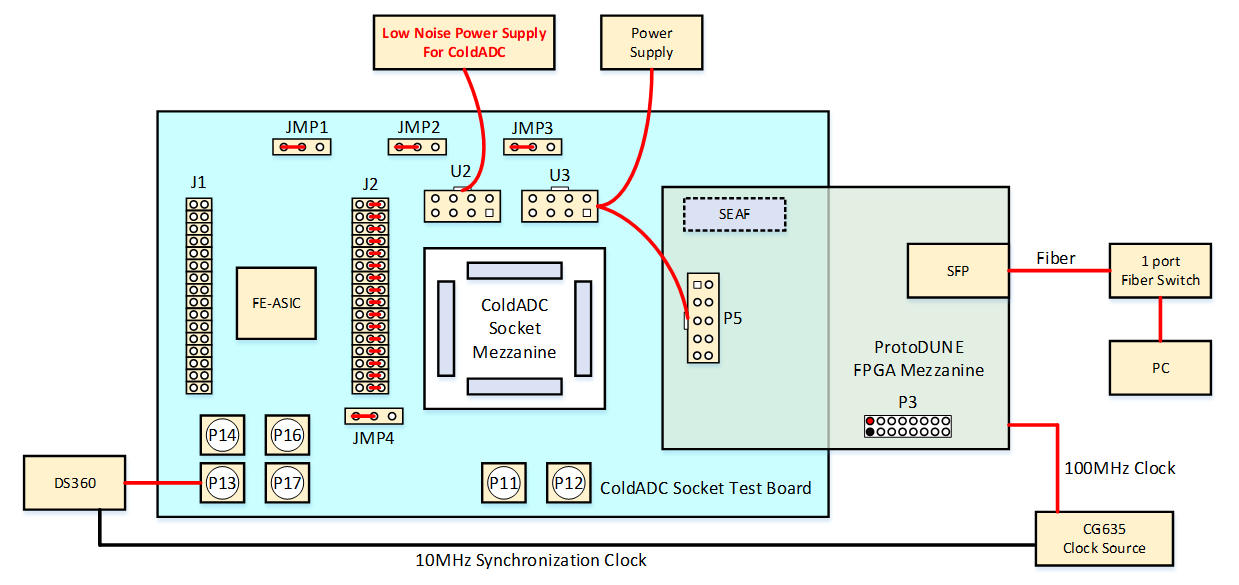
\includegraphics[width=0.8\linewidth]{figures/prodQC_blockdiagram.png}
  \caption{Block diagram of ColdADC Production Testing setup.}
  \label{fig:prodQC_blockdiagram}
\end{figure}

The flowchart of the QC process is shown Figure~\ref{fig:qc_flowchart}.  The chart illustrates the sequence of steps for characterizing 
the functionality and performance of the chip. At every iteration, the measurements is done using BJT reference and then repeated 
again using the CMOS reference. 
%With a certain number of tested chips, it will be possible to highlight differences in performance between measurements taken 
%using one reference instead of the other. 
%The test flow includes input configuration, initialization checkout, static linearity (INL/DNL per channel), 
%Dynamic Behavior (ENOB/SFDR/SINAD per channel), DC noise per channel, and ADC core characterization. 
The list below describes the QC steps in more detail: 
\begin{enumerate}
\item Input configuration: ColdADC chip ID and test board ID are recorded, the path for data storage is specified. 
\item Initialization checkout: mainly to check ColdADC functionality. It includes power consumption with different 
configurations, power cycles, I2C/UART communication check, pattern and register check, reference sweeping check, 
synchronization and calibration check. Any chip failed in any procedure in this checkout is treated as a bad chip. 
\item  Static linearity: INL/DNL results are obtained with a sine wave input from the DS360 generator. Data and plots 
are generated with the sine wave code-density method. Performances at both 2 MS/s/ch and 500 kS/s/ch are measured.
\item Dynamic Behavior: ENOB/SFDR/SINAD is calculated from the FFT plot obtained by using coherent sampling. 
Performances at both 2 MS/s/ch and 500 kS/s/ch are measured. 
\item DC noise: Two DC points, 200mV and 900mV are chosen.
\item ADC core characterization (optional): DNL/INL, FFT, and DC noise. 
\end{enumerate}

The test procedure is largely automated using Python scripts. The only step that requires manual intervention is to replace the ASIC chips 
at the end of the measurement. When the test is completed, the Python script automatically generates a detailed report in pdf format. 
The report includes:
\begin{enumerate}
\item Summary: date and time, temperature, chip and board IDs, power consumption and characterization results (CMOS reference only, can be changed to BJT);
\item Initialization checkout: ADC power consumption with both BJT and CMOS references, sweep plots of reference voltages and currents;
\item Calibration weights: recorded weights listed with respect to internal ADC stages;
\item Noise study: RMS noise for each channel and comparison between all channels. Four pages in total: 200 mV and 900 mV baselines for both BJT and CMOS references;
\item Channels characterization: noise, linearity and dynamic studies, with both BJT and CMOS references for comparison. Each page collects results for one channel;
\item ADC test input: internal ADC characterization for two sampling rates, 4 MS/s and 16 MS/s.
\end{enumerate}
\begin{figure}[h!]
\centering
  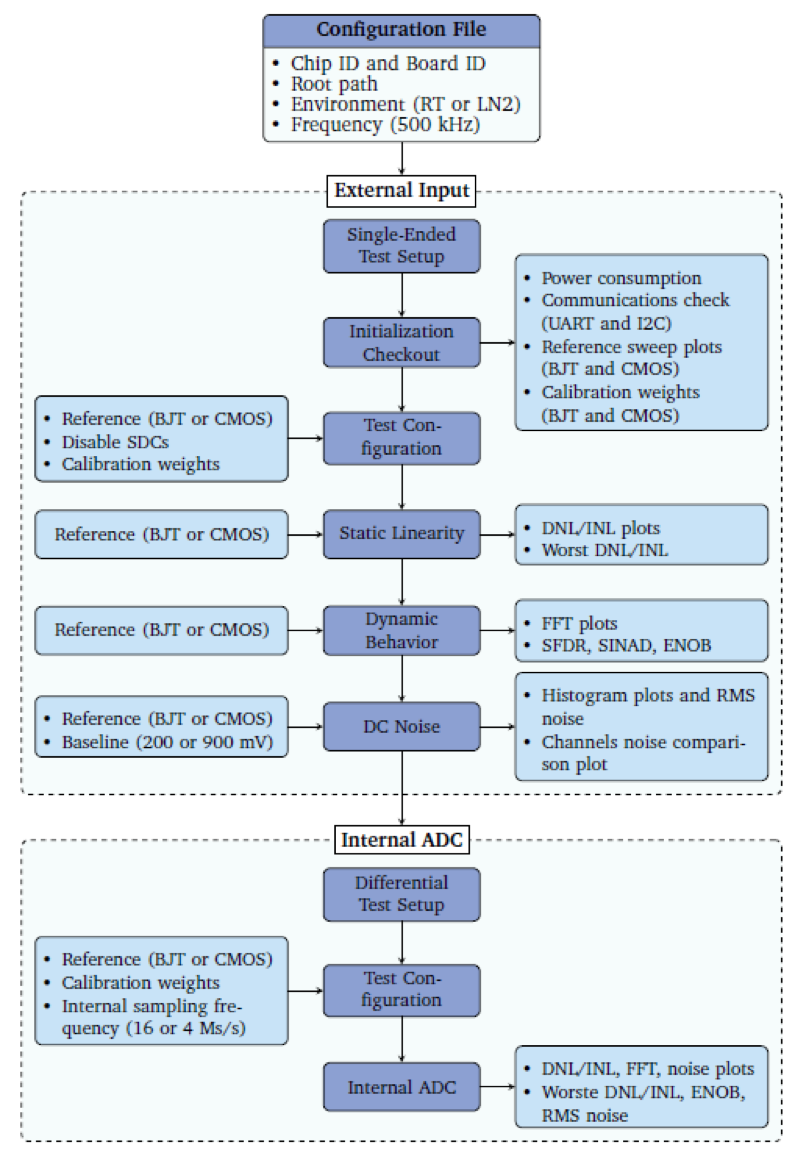
\includegraphics[width=0.8\linewidth]{figures/QC_flowchart.png}
  \caption{ColdADC QC Flowchart.}
  \label{fig:qc_flowchart}
\end{figure}

At the moment, the test data are stored in a local database at BNL. U. of Florida group is developing an online database for the ColdADC QC test that will be used for all future production tests.
%Ivan Furic research team from Florida University is going to develop an online database for the ColdADC QC test. BNL provides hardware, FPGA firmware, python scripts and necessary support to help them replicate the test procedure at BNL.  Florida University is responsible for QC test of 100 ColdADC chips in the coming two or three months. 

\subsection{Results}
\label{sec:6.2}
For the initial production QC test, a batch of 33 ColdADCs were tested. One of the chips (\#00096)  drew very high current (>1 A) when it 
was first powered and was excluded from further QC testing. It was found that the bad chip had a resistance of $<$ 5$\Omega$ between 
VDDA2P5 and VSSA2P5, while the nominal resistance should be about 12 k$\Omega$. The cause of the failure is not clear; may be due to 
manufacturing defect or handling issues. In additional to the 33 QC chips, 20 other chips were previously tested at BNL and passed 
functionality tests. Based on a sample of 53 chips (51 packaged and 2 bare dies), the functionality failure rate of ColdADC is less than 2\%.

\subsubsection{Power Consumption}
The power consumption of ColdADC strongly depends on the chip configuration. The power consumption with VDDA2P5/VDDD2P5=2.5V, 
VDDD1P2=2.1V, VDDIO=2.25V, SDC\&DB bypassed, CMOS reference, floating single-end input, and 2 MS/s sampling rate is summarized in in 
Figure~\ref{fig:qc_power}. For this configuration, the average power consumption of ColdADC is about 413 mW at room and 450 mW at LN$_2$ temperature.
\begin{figure}[h!]
\centering
  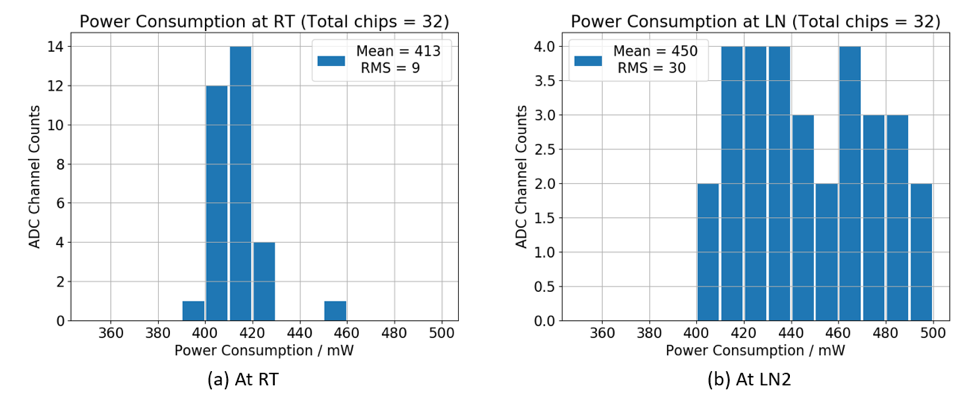
\includegraphics[width=0.85\linewidth]{figures/qc_power.png}
  \caption{Power consumption distribution.}
  \label{fig:qc_power}
\end{figure}

\subsubsection{Linearity Results with 2 Ms/s/channel Sampling Rate}
The results of the linearity and noise measurements at the nominal 2 Ms/s/channel sampling rate for the 33 chips are shown in 
FigureX (RT) and FigureY (LN$_2$). 
The QC tests are done with all 16 channels simultaneously connected to the signal source.
Due to the known SHA/MUX crosstalk issue, if the sample rate is 2MS/s per channel, the performance is expected to be worse. 
Another caveat is that the calibration of the ADC pipeline stages are not done for this result to shorten the testing cycle..
%The degradation is allowed because it is consistent to all chips, and additional test with 500 kS/s per 
%channel is also performed to confirm the degradation is caused by SHA/MUX crosstalk issue.  
%The ColdADC internally is 16-bit. The DUNE experiment requires 12-bit ADC is required by 
%DUNE experiment, ColdADC is truncated down to 12-bit by cut-off the lowest 4 bits. Meanwhile, in order to get ENOB, the coherency 
%frequency of sine wave is calculated for 12-bit ADC followed the equation of IEEE standard. 
Overall, the ColdADC performance is reasonably good, average of the worst DNL is 0.76LSB, average of the worst INL is 2.6LSB, 
average of ENOB is 10.0 bit and average of DC noise at 900mV is 0.68vLSB. In addition, the spread of these 4 key parameters 
among channels (or chips) is small.
Cryogenic test is performed as well with the same configuration,  Figure 7 shows the statistical result. 
By comparing Figure 6 and Figure 7, the linearity  performance of DNL, INL and ENOB do not show significant temperature dependence
 but the DC noise at LN$_2$ is smaller than at RT due to the suppression of thermal noise at cryogenic temperature.  


\newpage
\section{Summary}  
%	\input{summary}

\newpage
%\begin{thebibliography}{99}

%Citation from Introduction (Sec 1)
%

%
%Citation from Test Setup (Sec 2)
%

%
%Citation from Functional Testing (Sec 3)
%


%
%Citation from Performance Results (Sec 4)
%

%
%Citation from Issues Identified and Mitigations (Sec 5)
%


%
%Citation from Production Testing (Sec 6)
%


%
%Citation from Summary (Sec 7)
%


%
%Citation from Appendix
%



\bibitem{dunecdr} "LBNF/DUNE Conceptual Design Report",  \url{https://web.fnal.gov/project/LBNF/ReviewsAndAssessments/LBNF-DUNE\%20CD-1-Refresh\%20Directors\%20Review/SitePages/Conceptual\%20Design\%20Report.aspx}

\bibitem{montanari_35ton} First scientific application of the membrane cryostat technology, D.Montanari et al, \textit{AIP Proceedings 1573, 1664 (2014)} \url{http://scitation.aip.org/content/aip/proceeding/aipcp/10.1063/1.4860907}

\bibitem{genie} "The GENIE Neutrino Monte Carlo Generator", C. Andreopoulos, et al., Nucl. Instrum. Meth. A614, 87 (2010).



\end{thebibliography}



\newpage
\section*{Appendix}
%	\label{sec:appendix}




\end{document}
